\documentclass[tikz,border=5pt]{standalone}
\usepackage[osf]{libertine}
\begin{document}
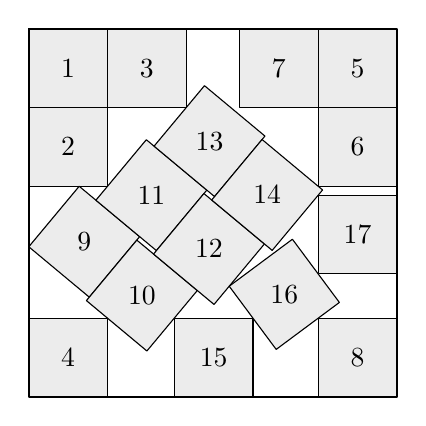
\begin{tikzpicture}[line cap=round,line join=round]
\foreach [count=\i]\x/\y/\angle in {
    0.5/4.17553009/0,
    0.5/3.17553009/0,
    1.5/4.17553009/0,
    0.5/0.5/0,
    4.17553009/4.17553009/0,
    4.17553009/3.17553009/0,
    3.17553009/4.17553009/0,
    4.17553009/0.5/0,
    0.70420216/1.97132794/50.19504102,
    1.43604349/1.28748666/50.19504102,
    1.55673716/2.56259422/50.19504102,
    2.28857850/1.87875294/50.19504102,
    2.29528645/3.24884655/50.19504102,
    3.02712778/2.56500527/50.19504102,
    2.34732483/0.5/0,
    3.24507371/1.30303623/36.62378638,
    4.17553009/2.06206996/0
  }{
    \begin{scope}[shift={(\x,\y)}, rotate=\angle]
      \draw[fill=gray!15] (-0.5,-0.5) rectangle (0.5,0.5);\node {\i};
    \end{scope}
  }
\draw[thick] (0,0) rectangle (4.67553009,4.67553009);
\end{tikzpicture}
\end{document}
